\documentclass[12pt, a4paper]{article} 
\usepackage[utf8]{inputenc} % codificação de strings
\usepackage[lmargin=3cm,tmargin=3cm,rmargin=2cm,bmargin=2cm]{geometry} % bordas ABNT
\usepackage[onehalfspacing]{setspace} % espaçamento 1.5cm
\usepackage[T1]{fontenc}
\usepackage[brazil]{babel}
\usepackage{graphicx, xcolor, comment, enumerate, multirow, multicol, indentfirst, hyperref} % Pacotes Essenciais
\usepackage{amsmath, amsthm, amsfonts, amssymb, dsfont, mathtools, blindtext} % Pacotes de Matemática

\title{Resumo do Artigo: A Deep Dense Neural Network for Bankruptcy Prediction}
\date{\today}

\begin{document}

\maketitle

\graphicspath{ {images/} }

\begin{itemize}
    \item Autores: Stamatios-Aggelos N. Alexandropoulos, Christos K. Aridas, Sotiris B. Kotsiantis, Michael N. Vrahatis
    \item Professora: Patrícia Romualdo de Almeida
    \item Aluno: Bruno Marcelino - 2019013155
\end{itemize}



\section{Introdução}

O objetivo do artigo é a aplicação de um modelo de Redes Neurais Artificiais (ANNs) na previsão de falência de empresas da bolsa da Grécia durante os anos de 2002 a 2004, a partir de uma amostra de 150 empresas.

Caso seja implementado, um modelo como esse pode ser interessante para qualquer tipo de credor, sendo passível de utilização tanto por entidades públicas que visam garantir um crescimento econômico sustentável das empresas, quanto grandes instituições financeiras que desejem incorporá-lo como gerenciamento de risco em suas operações de financiamento. 

\section{Classificação}

O trabalho realizado pode ser considerado uma pesquisa documental pelo fato de consolidar diversas informações relacionadas a projetos anteriores em um só artigo, que tem como base o resumo e citações às diversas formas de previsão já aplicadas por outros autores. Além disso, os autores ressaltam que os modelos gerados podem ser reelaborados a partir de estudos futuros, deixando claro que seus estudos ainda não receberam tratamento analítico suficiente para comprovar sua tese.

\section{Modelagem}

Redes Neurais Artificiais são modelos computacionais inspirados no Sistema Nervoso Central de um animal (em particular, o cérebro) e são capazes de realizar o aprendizado de máquina bem como o reconhecimento de padrões. Redes neurais artificiais geralmente são apresentadas como sistemas de "neurônios interconectados, que podem computar valores de entradas", simulando o comportamento das redes neurais biológicas. (Wikipedia)

O modelo utilizado pelo artigo em particular é do tipo mais simples de rede neural, conhecido como Perceptron Multicamadas (MLP). Nele, os neurônios funcionam como funções que recebem um vetor de inputs ($x_{1}, x_{2}, ..., x_{n}$) e retornam um vetor de outputs ($y_{1}, y_{2}, ...,y_{n}$), baseando-se em uma regra de cálculo específica.

\begin{figure}[h]
    \centering
    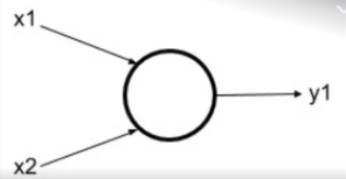
\includegraphics[scale = 0.75]{Screenshot_4} % sem espaços em branco ou muitos pontos
    \caption{Exemplo de Neurônio}
 %   \label{script} % declara a figura como uma variável
\end{figure}

No modelo MLP, cada neurônio realiza uma simples operação, que é definida como calcular uma função linear das variáveis (combinador linear) dado um viés (b) e pesos (w) para cada uma (Ex: $y = w_{1}x_{1} + w_{2}x_{2} + … + w_{n}x_{n}$). Logo depois, aplicamos uma função de ativação em cima do resultado obtido de forma que o resultado obtido seja um número entre 0 (solvência) e 1 (insolvência).

\begin{figure}[h]
    \centering
    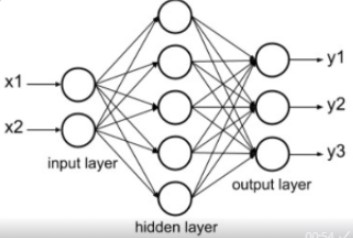
\includegraphics[scale = 0.75]{Screenshot_5} % sem espaços em branco ou muitos pontos
    \caption{Exemplo de Rede Neural}
    \label{script} % declara a figura como uma variável
\end{figure}

Para treinar uma rede neural, é criada uma função de custo que demonstra o quanto o valor previsto está distante do valor real desejado. Sendo “p” a probabilidade prevista de que Y = 1, a função retornará um valor “p” caso Y realmente seja 1 e “1-p” caso Y seja 0, penalizando a distância entre o valor previsto e o valor real. Ela estabelece uma recompensa com base em cada valor previsto pelo modelo (valor da verossimilhança) e retorna um score final para cada tipo de modelo estimado. O melhor modelo é o que maximiza a função de verossimilhança.

Para obter o melhor modelo possível, devemos alterar os valores dos pesos (w) e vieses (b) de cada neurônio de forma a obter o output desejado na maioria dos casos. Para isso, a rede neural MLP inicia esses coeficientes a partir de valores randômicos e tenta minimizar a função de custo de forma iterativa, até chegar em um ponto ótimo. O número de neurônios e camadas escondidas deve ser fornecido previamente.

\section{Resultados e Discussões}

Foram obtidos dados de 21 indicadores financeiros de cada empresa, e os autores fizeram questão de obter dados de duas empresas não-falidas para cada empresa falida, sendo que as três compartilham de dados similares e do mesmo setor. O modelo foi ajustado em um conjunto de treino e foram realizadas previsões no conjunto de teste, e abaixo estão os resultados obtidos.

\begin{figure}[h]
    \centering
    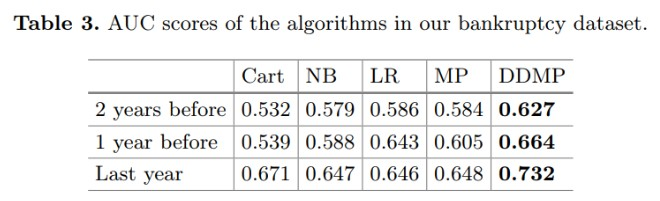
\includegraphics[scale = 0.75]{Screenshot_6} % sem espaços em branco ou muitos pontos
    \label{script} % declara a figura como uma variável
\end{figure}

Houve também bastante preocupação com relação ao overfitting, que é a perda da capacidade de generalização do modelo dada pelo ajuste perfeito à amostra de treinamento. Por isso os autores também utilizam de ferramentas para reduzir o peso de variáveis que podem ser pouco representativas.

\section{Conclusão}

Os resultados obtidos sugerem que o modelo de Redes Neurais foi o melhor dentre os seus pares mais utilizados em literaturas anteriores, logo há vasta oportunidade para que novas pesquisas envolvendo modelos de inteligência artificial sejam aplicadas, com o objetivo de tentar antecipar os eventuais riscos e prejuízos causados pela situação de insolvência de uma empresa.

\end{document}
